\section{Experiments}
\label{sec:experiments}

In the following sections we present the results of our experiments. For all simulated data
we generate our response vector according to \(\vec{y} = \mat{X}\vec{\beta}^* +
\vec{\varepsilon},\) with \(\vec{\varepsilon} \sim \normal(\vec{0}, \sigma_\varepsilon^2
\mat{I})\). We consider two types of features: binary (quasi-Bernoulli) and quasi-normal
features. To generate binary vectors, we sample \(\ceil{nq_j}\) indexes uniformly at random
without replacement from \([n]\) and set the corresponding elements to one and the
remaining ones to zero. To generate quasi-normal features, we generate a linear sequence
\(\vec{w}\) with \(n\) values from \(10^{-4}\) to \(1 - 10^{-4}\), set \(x_{ij} =
\cdf^{-1}(w_i)\), and then shuffle the elements of \(\vec{x}_j\) uniformly at random.

We use a coordinate descent solver to optimize our models, which we have based on the
algorithm outlined by \citet{friedman2010}. All experiments were coded using the Julia
programming language~\citep{bezanson2017} and the code is available at
% \url{https://github.com/jolars/normreg}.
in the supplementary material and will be published online upon acceptance.
%
All simulated experiments were run for at least 100 iterations and, unless stated
otherwise, are presented as means $\pm$ one standard deviation (using bars or ribbons).

\subsection{Normalization in Lasso and Ridge Regression}%
\label{sec:experiments-lassoridge}

In this section we consider fitting the lasso and ridge regression to normalized data sets.
To normalize the data, we standardize all quasi-normal features. For binary features, we
center by mean and scale by \(s_j \propto (q_j-q_j^2)^\delta\).

\subsubsection{Variability and Bias in Estimates}

% TODO: Where does this lambda setting come from? Is it the optimal setting?
In our first experiment, we consider fitting the lasso to a simulated data set with
\(n=500\) observations and \(p = \num{1000}\) features. The first 20 features correspond to
signals, with \(\beta_j^* = 1\), and otherwise we set \(\beta_j^*\) to 0. Furthermore, we
set the class balance of the first 20 features so that it increases geometrically from 0.5
to 0.99. For all other features we pick \(q_j\) uniformly at random in \([0.5,0.99]\). We
estimate the regression coefficients using the lasso, setting \(\lambda_1 = 2
\sigma_\varepsilon \sqrt{2 \log p }\), with \(\sigma_e\) set to achieve a signal-to-noise
ratio (SNR) of 2. In addition, we introduce correlation between the features by copying the
first \(\ceil{\rho n/2}\) values from the first feature to each of the following features.

The results~(\Cref{fig:binary-decreasing}) show that class balance has considerable effect,
particularly in the case of no scaling (\(\delta = 0\)), which corroborates our theory from
\Cref{sec:theory-binary-features}. At \(q_j=0.99\), for instance, the estimate
(\(\hat{\beta}_{20}\)) is consistently zero when \(\delta = 0\). For larger values of
\(\delta\), we see that class imbalance leads to increased estimation variance in
accordance with our theory for the orthogonal case. The effect of correlation appears to
have no effect on this class-balance bias, which indicates that the assumption of
orthogonality might not be necessary for our theory to hold.

\begin{figure}[htpb]
  \centering
  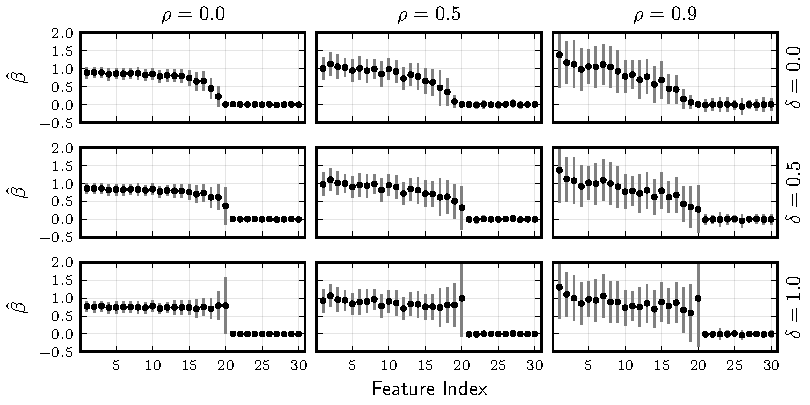
\includegraphics[]{binary_decreasing.pdf}
  \caption{%
    Regression coefficients for a lasso problem with binary data with \(n = 500\) and \(p =
    \num{1000}\). For \(j \in \{1,2,\dots,p\}\), we set \(\beta_j^* = 1\) and
    let \(q_j\) increase geometrically from 0.5 to 0.99. For the remaining features,
    we pick \(q_j\) uniformly at random from \([0.5, 0.99]\) and
    set \(\beta_j^* = 0\). We show only the first 30 coefficients.
  }
  \label{fig:binary-decreasing}
\end{figure}

\subsubsection{Predictive Performance}
\label{sec:experiments-predictive-performance}

In this section we examine the influence of normalization on predictive performance for
three different data sets: \data{rhee2006}~\citep{rhee2006}, and
\data{eunite2001}~\citep{chen2004}, and
\data{triazines}~\citep{hirst1994,king1995}.\footnote{See \Cref{sec:data-summary} for
  details about these data sets.} We present the results for lasso and ridge regression in
\Cref{fig:hyperopt-contours}, which shows contour plots of the validation set error in
terms of normalized mean-squared error~(NMSE). We see that optimal setting of \(\delta\)
differs between the different data sets: for \data{eunite2001}, both the lasso and ridge
are quite insensitive to the type of normalization, and low error is attainable for the
full range of \(\delta\). For \data{rhee2006}, this holds for the lasso too, but not for
ridge regression, where a value in approximately \([0,3]\) is optimal. Finally, for
\data{triazines}, the problem is quite sensitive to the choice of \(\delta\) as well as the
type of model used.

\begin{figure}[htpb]
  \centering
  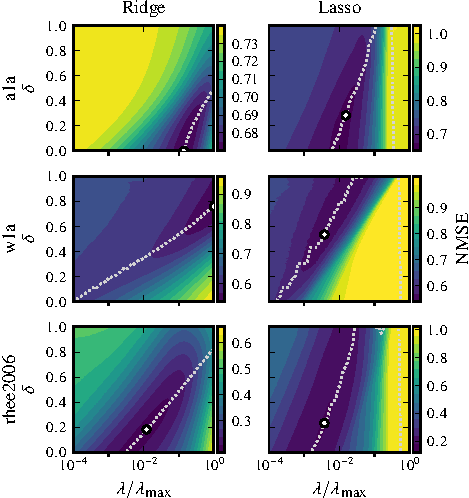
\includegraphics[]{hyperopt_surfaces.pdf}
  \caption{%
    Contour plots of normalized validation set mean-squared error (NMSE) for
    \(\delta\) and \(\lambda\) in lasso and ridge regression on three real data
    sets: \data{rhee2006}, \data{eunite2001}, and \data{triazines}. The dotted
    path shows the smallest NMSE as a function of \(\lambda\) and the circles
    mark combinations with the lowest error.
  }
  \label{fig:hyperopt-contours}
\end{figure}

Also see \Cref{sec:predictive-performance-support}, where we show how the support size of
the lasso solutions vary with \(\delta\) and \(\lambda\) and
\Cref{sec:predictive-performance-simulated}, where we complement these results with
experiments on simulated data under various class balances and signal-to-noise ratios,
again showing that normalization has a strong impact on predictive performance.

\subsubsection{Mixed Data}\label{sec:experiments-mixed-data}

In \Cref{sec:mixed-data} we discussed the issue of normalizing mixed data. Here, we examine
this issue empirically. We construct a quasi-normal feature with mean zero and standard
deviation 1/2 and a binary feature with varying class balance \(q_j\). We set the
signal-to-noise ratio to 0.5 and use \(n = \num{1000}\). These features are constructed so
that their effects are comparable under the notion of comparability that we introduced in
\Cref{sec:mixed-data} using \(\kappa = 2\). In order to preserve the comparability for the
baseline case when we have perfect class balance, we scale by \(s_j = 2 \times
(1/4)^{1-\delta}(q_j-q_j^2)^\delta\). Finally, we set \(\lambda\) to
\(\lambda_\text{max}/2\) and \(2\lambda_\text{max}\) for lasso and ridge regression
respectively.

The results~(\Cref{fig:lasso-ridge-comparison}) reflect our theoretical results from
\Cref{sec:theory}. In the case of the lasso, we need \(\delta =1\) (variance scaling) to
avoid the effect of class imbalance, whereas for ridge we instead need \(\delta =1/2\)
(standardization). As our theory suggests, this extra scaling mitigates this class-balance
bias at the cost of added variance.

\begin{figure}[htpb]
  \centering
  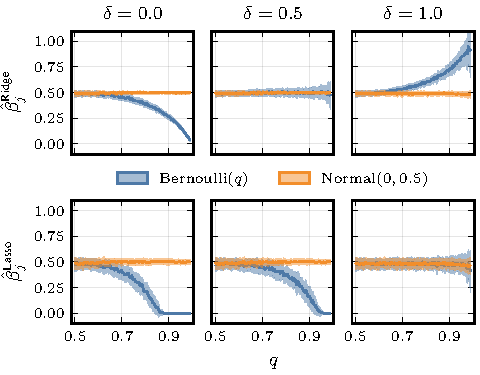
\includegraphics{mixed_data.pdf}
  \caption{%
    Lasso and ridge estimates for a two-dimensional problem where one feature is a binary
    feature with class balance \(q_j\) (\(\bernoulli(q_j)\)) and the other is quasi-normal
    with standard deviation 1/2, (\(\normal(0, 0.5)\)).
  }
  \label{fig:lasso-ridge-comparison}
\end{figure}

\subsubsection{Interactions}\label{sec:experiments-interactions}

Next, we study the effects of normalization and class balance on interactions in the lasso.
Our example consists of a two-feature problem with an added interaction term given by
\(x_{i3} = x_{i1}x_{i2}\). The first feature is binary with class balance \(q\) and the
second quasi-normal with standard deviation 0.5. We use \(n=1000\), \(\lambda_1 = n/4\),
and normalize the binary feature by mean-centering and scaling by \(\kappa (q - q^2)\),
using \(\kappa = 2\). We consider two different strategies for choosing \(s_3\): in the
first strategy, which we call \emph{Strategy 1}, we simply standardize the resulting
interaction feature. This is a common strategy used, for instance in
\citet{bien2013,lim2015}. In the second strategy, \emph{Strategy 2}, we center with mean
and scale with \(s_1s_2\) (the product of the scales of the binary and normal features).

The results~(\Cref{fig:interactions}) show that only Strategy 2 estimates the effect of the
interaction correctly. Strategy 1, meanwhile, only selects the correct model if the class
balance of the binary feature is close to 1/2 and in general shrinks the coefficient too
much.

\begin{figure}[htpb]
  \centering
  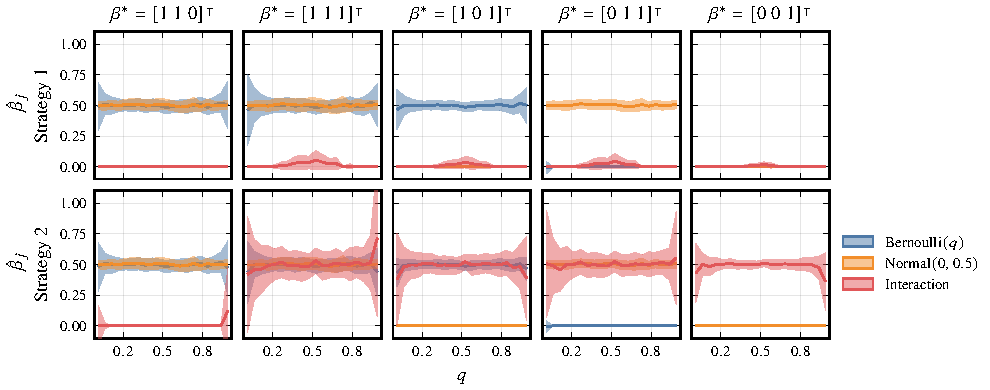
\includegraphics[]{interactions-classbalance.pdf}
  \caption{%
    Lasso estimates for a problem with a binary feature, a quasi-normal
    feature, and an interaction feature. We have varied the true signal
    \(\bm{\beta}^*\) and use two different normalization strategies for the
    interaction, where
    Strategy 1 represents standardization and Strategy 2 is mean-centering
    together with scaling by \(s_1 s_2\).
  }
  \label{fig:interactions}
\end{figure}

\subsection{The Weighted Elastic Net}

The weighted elastic net can be used as an alternative to normalization to correct for
class balance bias when \(\lambda_1 > 0\) and \(\lambda_2 >0\). To simplify the
presentation, we parameterize the elastic net as \(\lambda_1 = \alpha \lambda \) and
\(\lambda_2 = (1-\alpha) \lambda\), so that \(\alpha\) controls the balance between the
ridge and lasso. We conduct an experiment with the same setup as in
\Cref{sec:experiments-mixed-data}, but here we use the weighted elastic net instead with
\(\alpha = 0.5\). We use \(n=1000\) and vary \(\omega\), using the weights \(u_j = v_j =
(q_j - q_j^2)^{\omega}\) as we suggested in \Cref{sec:binary-weighting}. Our results
(\Cref{fig:mixed-data-elnet}) show that \(\omega = 1\) leads to seemingly unbiased
estimates.

\begin{figure}[htpb]
  \centering
  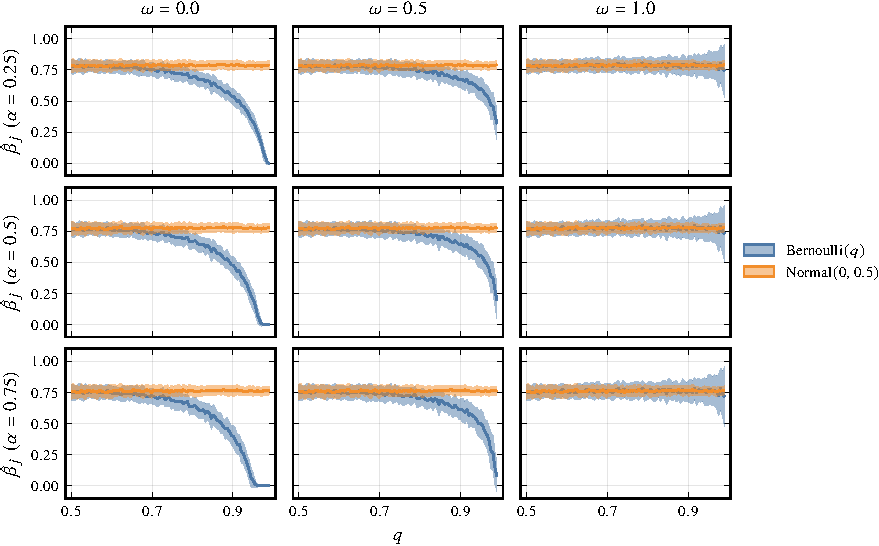
\includegraphics{mixed_data_elnet.pdf}
  \caption{%
    Weighted elastic net estimates for \(\alpha = 0.5\) for a problem with a binary
    feature with class balance \(q\) (\(\bernoulli(q)\)) and quasi-normal
    with standard deviation 1/2 (\(\normal(0, 0.5)\)). \(\omega\) indicates
    the scaling of the penalty weights.
  }
  \label{fig:mixed-data-elnet}
\end{figure}

\subsection{Additional Results}

In \Cref{sec:additional-experiments} we present extended results of our experiments as well
as several additional experiments. For instance, we also consider an experiment on the
Boston housing data set in \Cref{sec:dichotomization}, where we try to estimate the effect
of normalization on dichotomized versions of the features and find that \(\delta = 1\)
leads to feature ranks that best correspond to the linear regression solution.
